% !TEX root = mythesis.tex

%==============================================================================
\chapter{Statistical Methods and Analysis Setup}

%==============================================================================

In particle physics, the abundance of available data for exploration has dramatically increased with the development of 
powerful particle colliders. Be it estimating a parameter of the SM or finding
evidence of new physics, particle physicists heavily rely on statistical techniques to churn
out reliable information from observed data. This chapter provides details on the statistical methods
used in this thesis. Basic statistical techniques including parameter 
estimation and method of maximum likelihood are outlined in \cref{sec:statinfer}.
The concept of unfolding is introduced and the techniques used in this thesis are explained in
detail. This chapter also discusses the method of profile likelihood 
unfolding, which is the core technique used in this analysis.

\section{Statistical Inference}
\label{sec:statinfer}
The main goal of a statistical analysis is to infer key information from the observed data.
Commonly used approaches of inference are frequentist and Bayesian which are based on the
interpretation of probability. In statistics, probability is simply the "chance" of an event ocurring.
In the frequentist approach, probability is interpreted as the 
frequency of an event occurring, whereas in the Bayesian approach, probability is the extent of 
belief in the occurrence of an event~\cite{2015arXiv150400945P}. 

Statistical problems can be categorised into two types: parameter estimation and hypothesis 
testing. In parameter estimation, the goal is to determine the "best" possible value of a certain
physical quantity or a parameter of a certain mathematical model. It is important to note that 
the parameter value is always accompanied by an error estimate which quantifies the accuracy of 
a measurement. A measurement may not be perfect, however the extent of imperfection is 
concealed in the error values. Therefore, error values play an important role in the interpretation of 
experimental results.

In hypothesis testing, the main goal is to check if a theory is consistent with the observed data.
For this case, the answer is not a numerical value, instead, it is a statement implying 
how confident we are with the consistency of a theory based on the observed data. In reality,
hypothesis testing and parameter estimation are not totally independent of each other. 
Some problems require estimating a parameter in order to test a hypothesis while in some cases, 
a parameter is estimated assuming a hypothesis is correct~\cite{Lyons_1986}. In this analysis,
we focus on parameter estimation. In frequentist statistics, method of least squares and 
method of maximum likelihood are mainly used for parameter estimation. In this thesis, the maximum likelihood 
method is used which is discussed in the next section. 

\subsection*{Method of maximum likelihood}

Statistical models are mathematical expressions that relate observations to underlying theories.
These models are characterised by a set of parameters. The possibilities of different outcomes, 
given a mathematical model, is described by probabilities which is a key concept in statistics.
Another important concept which connects observations to parameters, is the likelihood.
Likelihood is a measure of how likely a set of parameters can describe the actual observed data. 
% Here, the observed data are fixed, while the parameters are unknown, making this approach 
% conceptually opposite to the definition of probabilities. 

Consider a random variable $x$ distributed according to a probability distribution function $f(x;\theta)$
where $f(x;\theta)$ represents our assumed hypothesis. Now suppose the functional form of $f(x;\theta)$ 
is known, however, some parameters are unknown. Suppose a measurement is performed yielding $n$ independent
values, denoted by ${x_1,x_2,...,x_n}$.  The probability of observing this particular set of values 
is given by the product of the individual probabilities for each value, as given in \cref{eqn:prob}. 

\begin{equation}
    P (x_1,x_2,...,x_n,\theta) = \prod_{i=1}^{n} f (x_i,\theta)dx_i
    \label{eqn:prob}
\end{equation}

If the assumed hypothesis is correct, the probability of observing the data should to be high. 
This concept leads to the \textit{likelihood function} $L(\theta)$, which is defined as:

\begin{equation}
    L (\theta) = L(\theta | x_1,x_2,...,x_n) = \prod_{i=1}^{n} f (x_i,\theta)dx_i
    \label{eqn:likeli}
\end{equation}


Here, $L(\theta)$ measures how likely it is to observe the set ${x_1,x_2,...,x_n}$, given the 
parameter $\theta$. Unlike a standard probability function, the likelihood function treats the 
data as fixed and considers $\theta$ as the variable.

The objective of maximum likelihood estimation is to find the value of 
$\theta$ that makes the observed data most probable. In other words, we search for the parameter 
values that maximize the likelihood function, a process referred to as the method of maximum 
likelihood or maximum likelihood fitting. In practice, it is often more convenient to maximize the 
logarithm of the likelihood function, known as the log-likelihood. This transformation simplifies the 
product of probabilities in the likelihood function into a sum, which is mathematically easier to 
handle while preserving the location of the maximum.
\mynote[inline]{}{explain profile-likelihood}

The method of maximum likelihood depends on the observed data. The efficiency of parameter determination
will depend on the extent of reliability on observed data. In particle physics, this fact imposes a 
certain level of expectations from particle detectors. Even though our detectors are well-developed
and efficient, there are some limitations that lead to distortion of observations. Physicists often use
mathematical techniques to remove the distortions caused by detectors. These techniques fall under the
category of \textit{unfolding}.  

\section{Basic concept of unfolding}

In any experiment, the accuracy of measurement depends heavily on the performance of the apparatus 
used. In particle physics, an ideal detector would capture the original and complete information 
of collisions without any loss or distortion, accurately preserving the true shape
of distributions for any physical observable. However, in reality, the data received 
from a detector is distorted due to effects such as limited acceptance and 
finite resolution of the detector. These distortions may lead to incorrect inferences and
therefore, need to be removed.

Unfolding is a mathematical technique used to remove distortions and estimate the original
fine structure of detector data. This technique is also called desmearing or deconvolution.
In unfolding, the goal is to estimate the true distribution from the observed distribution, 
using a response matrix. The response matrix is a mathematical construct that 
characterises the smearing effects introduced by the detector. An illustration visualising 
unfolding is shown in \cref{fig:unf_graphic}.

Unfolding is essential in various contexts. For instance, it enables results to be 
combined or compared with those from other experiments that may have different 
levels of smearing. Additionally, it is not always practical to present results alongside 
their response matrices. Unfolding becomes crucial when comparing experimental 
results directly to theoretical predictions without accounting for experimental 
distortions. Furthermore, non-distorted data is needed when fitting specific parameters to 
data for tuning Monte Carlo simulations~\cite{Lyons:2011cli}.


\section{Unfolding methodology}

There are certain conventions regarding the entities used in unfolding problems within the particle physics 
community. The distribution of a physical observable obtained from data recorded by the detector is called detector-level 
distribution. On the other hand, the truth-level distribution represents data that we should
have obtained with an ideal detector. This is generated from MC simulations without applying any detector
simulations. In unfolding, we also make use of simulated distribution including detector simulation.
Since this so-called reconstructed-level distribution is supposed to mimic actual observed data, it is 
used to validate an unfolding method. Detector-level and reconstructed-level distributions are 
conceptually the same when discussing unfolding related quantities. Technically, unfolding
is a method of estimating the truth-level by correcting detector effects present at detector- or
reconstructed-level.

\begin{figure}
    \centering
        \includegraphics[width=\textwidth]{unfolding_graphic.jpg}
        \caption{An illustration visualising the method of unfolding. The left diagram is an illustration
        of a histogram obtained from the detector information, called detector-level and the right 
        illustration shows a histogram that is expected form an ideal detector, called truth-level.
        The difference in the two diagrams depicts the smearing caused by the detector. The procedure to
        obtain the truth-level information based on the detector-level information is called as 
        unfolding. The reverse procedure is called folding.}
           \label{fig:unf_graphic}
  \end{figure}

The reconstructed distribution $\vec{x}$ is related to the truth-level distribution $\vec{y}$ by
a response matrix $R$ as shown in \cref{eqn:unfmath}. Here $\vec{b}$ represents backgrounds. In particle physics problems, data is 
generally organised into histograms with finite bins. In this case the above given relation 
is given by \cref{eqn:unfmath2}.


\begin{equation}
    \vec{x} = R \cdot \vec{y} + \vec{b}
    \label{eqn:unfmath}
\end{equation}

\begin{equation}
    x_i = \sum_{\text{j = 1}}^{\text{bins}} \mathcal{R}_{ij} y_j + \vec{b}
    \label{eqn:unfmath2}
\end{equation}

A response matrix which quantifies the detector effects is computed from simulated data. 
The quantities used to construct the response matrix are migration matrix and two correction 
factors namely acceptance and efficiency. A schematic showing reconstructed-level
and fiducial truth-level volumes is given in \cref{fig:recotruth}.
Per-bin acceptance adjusts the number of reconstructed
events by the fraction of events that are also present at the fiducial truth-level. It is defined 
as the ratio of events present at the reconstruction- and truth-levels to the total number of 
events at the reconstruction-level. Acceptance gives an idea of how well the reconstructed data
corresponds the true data. The corrected number of events at the reconstructed-level is
given as,

\begin{equation}
    N_{i}^{\text{reco}} = x_i * a_i
\end{equation}

Per-bin efficiency adjusts the number of truth-level events by the fraction of truth-level events
that are also found at the reconstructed-level. It is defined as the ratio of a number of events
present at both the reconstruction-level and the truth-level to the total number of events at the 
fiducial truth-level. This correction factor gives an idea of the detector's efficiency to 
reconstruct true events. The corrected number of events at the fiducial truth-level is
given as,

\begin{equation}
    N_{j}^{\text{fid}} = y_j * \epsilon_j
\end{equation}

The migration matrix describes the bin-to-bin migrations between truth-level and 
reconstruction-level histograms. For instance, $M_{ij}$ represents the fraction of events 
found in bin $i$ at the reconstruction-level while being created in bin $j$ at the truth-level.
A migration matrix with maximum diagonal components indicates that most events are 
reconstructed in the same bin in which they were generated. \Cref{eqn:unfmath2} can be re-written as,

\begin{equation}
    N_{i}^{\text{reco}} = \frac{a_i}{\epsilon_j} * \sum_{\text{j = 1}}^{\text{bins}} M_{ij} \cdot N_{j}^{\text{fid}} 
\end{equation}


\begin{figure}
    \centering
        \includegraphics[width=0.6\textwidth]{recotruth.jpg}
        \caption{A schematic picture showing reconstructed-level volume in blue and 
        truth-level volume in pink.}
           \label{fig:recotruth}
  \end{figure}

Mathematically, the idea of unfolding is to solve \cref{eqn:unfmath} for given 
$\mathcal{R}$, $x$ and $b$. The resultant values of $y$ can be interpreted as 
determined true number of events at the truth-level. One would notice a simple way to 
find the estimators by inverting the response matrix as shown in \cref{eqn:invert}.

\begin{equation}
    \vec{y} = \mathcal{R}^{-1} (\vec{x}-\vec{b})
    \label{eqn:invert}
\end{equation}

Although matrix inversion method is easy to implement, it is a strategy that one should 
avoid because of its limitations: in some situations, the response matrix is non-invertible
then \cref{eqn:invert} becomes ill-posed. Even though inversion is possible, there are possible
statistical fluctuations in the observed data that may cause negative entries in the 
inverse matrix. This leads to negative number of events in the unfolded distribution
which is unrealistic. When a response matrix acts on a true spectrum, it distorts any 
fine structure present at the truth-level. Despite that, some residue of this fine 
structure still remains in the reconstructed spectrum~\cite{cowan}. The inverted matrix, 
acting on the measured data, assumes its statistical fluctuations are the residual fine 
structure and restores it. In this way, statistical fluctuations are amplified in the unfolded
distribution~\cite{inverse} which is undesirable.

In order to overcome the limitations of matrix inversion, alternate unfolding methods are used
in high energy physics. Some of the methods are summarised in~\cite{refId0}.
In this thesis, the iterative Bayesian unfolding (IBU) and profile-likelihood unfolding (PLU)
are discussed.



\section{Iterative Bayesian unfolding (IBU)}

D'Agostini~\cite{DAGOSTINI1995487} proposed a method called iterative Bayesian unfolding (IBU) 
which makes use of Bayes' theorem. To describe this method, consider true events as 
\textit{causes} ($C_i, i=1,2,...,n_C$) and reconstructed events as 
\textit{effects} ($E_j, j=1,2,...,n_j$). The conditional probability that a cause $C_i$ gave 
rise to effect $E_j$, denoted by $P(C_i|E_j)$, is given by Bayes' theorem:

\begin{equation}
    P(C_i|E_j) = \frac{P(E_j|C_i)P(C_i)}{P(E_j)} 
    \label{eqn:5.14}
\end{equation}
where, $P(E_j|C_i)$ can be interpreted as probability of reconstructed event given true 
event which is the element $M_{ij}$ of the migration matrix. Consequently, $P(C_i|E_j)$ can 
be identified as the unfolding matrix. One can determine the number of events ($\hat{n}$) 
due to cause $C_i$ as

\begin{equation}
    \hat{n}(C_i) = \frac{1}{\hat{\epsilon_i}}\sum_{j=1}^{n_E} \hat{n}(E_j) P(C_i|E_j).
    \label{eqn:5.15}
\end{equation}

It is important to note that the total number of events due to all causes and all 
effects are equal because only migration effects are considered so far. By dividing both 
the sides of Equation~\ref{eqn:5.15} by total number of events, we obtain

\begin{equation}
     P(C_i) = \frac{1}{\hat{\epsilon_i}}\sum_{j=1}^{n_E}P(E_j) P(C_i|E_j).
     \label{eqn:5.16}
\end{equation}
Here, $P(C_i)$ is the unfolded distribution. This technique is implemented in the 
\texttt{RooUnfold}~\cite{roounfold} software package. The steps performed in iterative Bayesian 
unfolding to find $P(C_i)$, are shown in Figure~\ref{fig:5.3} and explained below:
\begin{itemize}
    \item An initial guess $P_0(C_i)$ is made and inserted into Equation~\ref{eqn:5.16}. $P(E_j)$ is obtained from MC reconstructed distribution. The solution provides $P(C_i|E_j)$ which is the unfolding matrix.
    \item The obtained $P(C_i|E_j)$ is used in Bayes' theorem (Equation~\ref{eqn:5.14}) to get a value of $P(C_i)$ which is different from the initial guess.
    \item This process is repeated for number of iterations specified by user. 
\end{itemize}


\begin{figure}
    \centering
    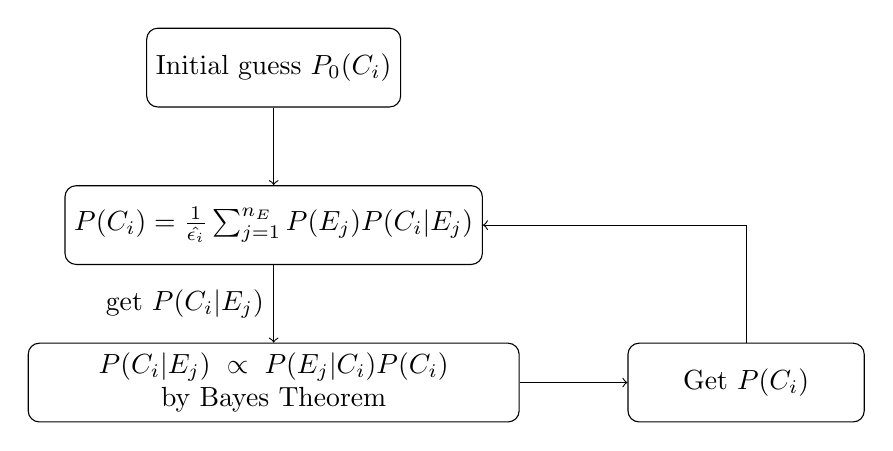
\begin{tikzpicture}[node distance=2cm]
    \tikzstyle{startstop} = [rectangle, rounded corners, minimum width=3cm, minimum height=1cm,text centered, draw=black]
    \node (start) [startstop] {Initial guess $P_0(C_i)$};
    \tikzstyle{io} = [rectangle, rounded corners, minimum width=3cm, minimum height=1cm,text centered, draw=black]
    \node (in1) [io, below of=start] {$P(C_i) = \frac{1}{\hat{\epsilon_i}}\sum_{j=1}^{n_E} P(E_j) P(C_i|E_j)$}; 
    \tikzstyle{process} = [rectangle, rounded corners, minimum width=3cm, minimum height=1cm,text centered,text width=6 cm, draw=black]
    \node (pro1) [process, below of=in1] {$P(C_i|E_j)\propto P(E_j|C_i) P(C_i)$ by Bayes Theorem};
    \tikzstyle{decision} = [rectangle, rounded corners, minimum width=3cm, minimum height=1cm,text centered, draw=black]
    \node (dec1) [decision, right of=pro1, xshift=4 cm] {Get $P(C_i)$};
    \draw [->] (start) -- (in1);
    \draw [->] (in1) -- node[anchor=east] {\textcolor{black}{get $P(C_i|E_j)$}} (pro1);
    \draw[->] (pro1) -- (dec1);
    \draw [->] (dec1) |-  (in1);
    
    \end{tikzpicture}
    \caption{Flow chart showing steps followed in iterative Bayesian unfolding }
    \label{fig:5.3}
    \end{figure}

\section{Profile-likelihood fitting and unfolding}

Profile-likelihood unfolding (PLU) is a method where the unfolding problem is translated into a 
likelihood maximisation problem. In PLU, a profile-likelihood fit is performed to estimate the 
underlying parameters which are then used to estimate the true distribution. 